\documentclass{article}

\title{Outcome Gaps in Higher Education}
\author{Xiaoqian Zhu, Shirley Jin, Tina Huang, Abigail Chaver}
\date{\today}

\usepackage{amsmath}
\usepackage{graphicx}
\usepackage[margin=0.75in]{geometry}
\usepackage{float}
\usepackage{hyperref}
\usepackage{wrapfig}

\usepackage{Sweave}
\begin{document}
\Sconcordance{concordance:report.tex:/Users/Abigail/Documents/stat159-project3/stat159-project3/reports/report.Rnw:%
1 13 1 1 0 4 1 1 8}
\Sconcordance{concordance:report.tex:/Users/Abigail/Documents/stat159-project3/stat159-project3/reports/sections/01-Abstract.Rnw:ofs 20:%
1 5 1}
\Sconcordance{concordance:report.tex:/Users/Abigail/Documents/stat159-project3/stat159-project3/reports/report.Rnw:ofs 26:%
28}
\Sconcordance{concordance:report.tex:/Users/Abigail/Documents/stat159-project3/stat159-project3/reports/sections/02-Introduction.Rnw:ofs 27:%
1 10 1}
\Sconcordance{concordance:report.tex:/Users/Abigail/Documents/stat159-project3/stat159-project3/reports/report.Rnw:ofs 38:%
30}
\Sconcordance{concordance:report.tex:/Users/Abigail/Documents/stat159-project3/stat159-project3/reports/sections/03-Data.Rnw:ofs 39:%
1 22 1}
\Sconcordance{concordance:report.tex:/Users/Abigail/Documents/stat159-project3/stat159-project3/reports/report.Rnw:ofs 62:%
32}
\Sconcordance{concordance:report.tex:/Users/Abigail/Documents/stat159-project3/stat159-project3/reports/sections/04-eda.Rnw:ofs 63:%
1 65 1}
\Sconcordance{concordance:report.tex:/Users/Abigail/Documents/stat159-project3/stat159-project3/reports/report.Rnw:ofs 129:%
34}
\Sconcordance{concordance:report.tex:/Users/Abigail/Documents/stat159-project3/stat159-project3/reports/sections/05-anova.Rnw:ofs 130:%
1 1 1 1 4 4 1 1 4 12 0 1 2 10 1 1 8 11 0 1 2 2 1 1 8 11 0 1 2 7 1}
\Sconcordance{concordance:report.tex:/Users/Abigail/Documents/stat159-project3/stat159-project3/reports/report.Rnw:ofs 196:%
36}
\Sconcordance{concordance:report.tex:/Users/Abigail/Documents/stat159-project3/stat159-project3/reports/sections/06-second-model.Rnw:ofs 197:%
1 14 1 1 7 1 1 1 5 17 0 1 3 9 1 1 5 17 0 1 3 13 1}
\Sconcordance{concordance:report.tex:/Users/Abigail/Documents/stat159-project3/stat159-project3/reports/report.Rnw:ofs 274:%
38 2 1}
\Sconcordance{concordance:report.tex:/Users/Abigail/Documents/stat159-project3/stat159-project3/reports/sections/07-random_forest.Rnw:ofs 277:%
1 6 1 1 5 1 1 1 22 22 0 1 2 36 1}
\Sconcordance{concordance:report.tex:/Users/Abigail/Documents/stat159-project3/stat159-project3/reports/report.Rnw:ofs 346:%
42}
\Sconcordance{concordance:report.tex:/Users/Abigail/Documents/stat159-project3/stat159-project3/reports/sections/08-Conclusion.Rnw:ofs 347:%
1 11 1}
\Sconcordance{concordance:report.tex:/Users/Abigail/Documents/stat159-project3/stat159-project3/reports/report.Rnw:ofs 359:%
44 1 1}


\maketitle


% !Rnw root = report.Rnw
\section{Abstract}

In this report, we investigate "outcome gaps" in higher education - the widespread phenomenon that underrepresented students have worse outcomes than their well-represented peers. Using data from College Scorecard, a federally maintained dataset, we explore the differences between completion rates across races, and differences between post-graduation earnings across parent-income terciles.

We test the hypotheses that the type of school (public, non-profit private, or for-profit private) and the instructional expenditure per full-time student are related to outcome gaps, finding statistically significant relationships in both cases. We also run a random forest regression across 14 other possible explanatory factors to provide some insight on possible interactions. The random forest model was not particularly useful as a predictor, but provided some interesting suggestions as to what circumstances correspond to worse outcome gaps.

% !Rnw root = report.Rnw

\section{Introduction}

We are interested in factors that are related to "outcome gaps" for students in higher education. Our high-level goal is to identify factors which are associated with under-represented students having a higher degree of difficulty succeeding than their well-represented peers. We are investigating this issues partly from the perspective as students attending a public school, UC Berkeley, with great resources compared to other public schools, but less compared to private schools at similar levels of selectivity. We are attempting to provide a data-based analysis of the theory that underrepresented students struggle more in comparison to their peers when attending institutions that have fewer resources to support them. 

Given that there is a major social-good imperative to decrease these outcome gaps, we hope that this analysis can provide hard evidence that there are patterns to the degree of outcome inequality. Specifically, we are interested in the question of whether additional government investment in public education can decrease outcome gaps. Obviously, it is impossible to conduct an experiment to answer this question and justify any kind of causal relationship, but with thorough investigation we hope to provide strong evidence that this pattern is consistent enough to be taken seriously by policymakers.

Since expenditures are also highly correlated with other factors - for example, there is no accounting for the higher cost of living in coastal and urban regions - it is worthwhile to consider some additional factors to see whether interactions between factors are related to outcome gaps. Running a random forest model will allow us to get some sense of which variables are most important for predicting outcome gaps. This broader view of what might be related to outcome gaps should provide more insight into how we can address the problem.



% !Rnw root = report.Rnw

\section{Data}

\subsection{Source}

We began by looking at the available data from College Scorecard, available at \url{https://collegescorecard.ed.gov/}, which contains data on over 7500 higher education institutions in the US. College Scorecard has an API that can handle complicated filtered requests, but we downloaded the full dataset to have full flexibility in exploration. College Scorecard provides a data dictionary to comb through the thousands of variables it provides.

\subsection{Target Variables}

We found that completion rates were disaggregated by race, and post-graduation earnings were disaggregated by parent-income terciles. Therefore, we computed outcome gaps for these two statistics according to the cohorts provided. We compared white completion rates to black, hispanic, and Asian completion rates, defining the outcome gap with the equation 
$$[(White Completion Rate) - (Minority Completion Rate)]/ (White Completion Rate)$$
For earnings gaps, we have ordered terciles, so we compute
$$[(Higher Tercile Earnings) - (Lower Tercile Earnings)]/ (Higher Tercile Earnings)$$

While computing these outcome statistics, we found inevitably that we got some were incomputable. This was particularly common with historically black schools, where the completion rate for white students was not recorded or recorded as zero. Therefore, we excluded such observations from our data set, as we are interested in cases where we can compare outcomes between white students and students of color.

\subsection{Explanatory Variables}

We found that College Scorecard provided two explanatory variables that were useful for our analysis, "CONTROL", a coded variable representing whether the school is under control of the government, a corporation, or a non-profit. The dataset also provided "INEXPFTE", Instructional Expenditures per Full-Time Student. This is an excellent proxy variable for a quantifier of the resources a school provides to its students.

In the third part of our analysis where we consider additional exploratory variables and their interactions, we used our best judgment to choose possible relevant variables. Our random forest regression uses variables related to the type of degree awarded, the region and type of location, the admission rate, the proportion of students of each of the four races considered, the median cost to attend, the median household income, and the poverty rate.



% !Rnw root = report.Rnw

\section{Exploratory Data Analysis}

Our final dataset, after omitting null values, was around 2000 observations. We wanted to begin our informal analysis by plotting some data from schools with which are familiar. Therefore, we considered three cohorts - the California State University schools, the University of California schools, and the elite private schools, comprised of the Ivies and a few others. We actually considered a fourth cohort, the top-expenditure schools, but those mostly overlapped with the third cohort.

\begin{figure}[H]
\centering
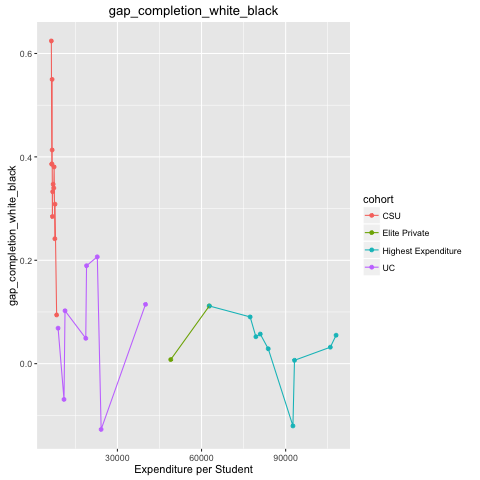
\includegraphics[width=0.3\textwidth]{../images/eda_scatterplots/gap_completion_white_black_cohort.png}
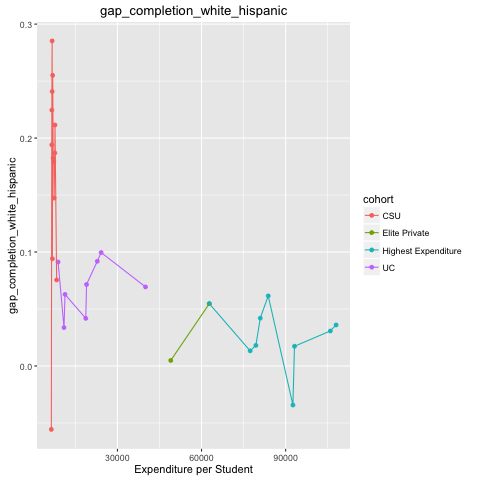
\includegraphics[width=0.3\textwidth]{../images/eda_scatterplots/gap_completion_white_hispanic_cohort.png}
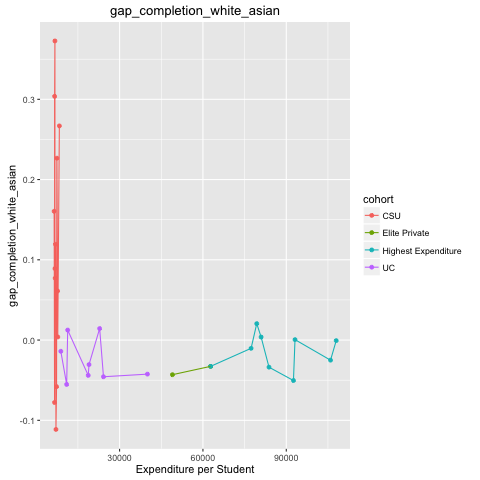
\includegraphics[width=0.3\textwidth]{../images/eda_scatterplots/gap_completion_white_asian_cohort.png}
\caption{\label{fig: CompletionRatesCohorts} We see that while there is a clear segmentation of expenditures across cohorts, the difference in outcomes is not as clear-cut. There is a general negative relationship, but a lot of variance. The most obvious conclusion is that the CSUs suffer from much worse outcome gaps than the other cohorts.}
\end{figure}

\begin{figure}[H]
\centering
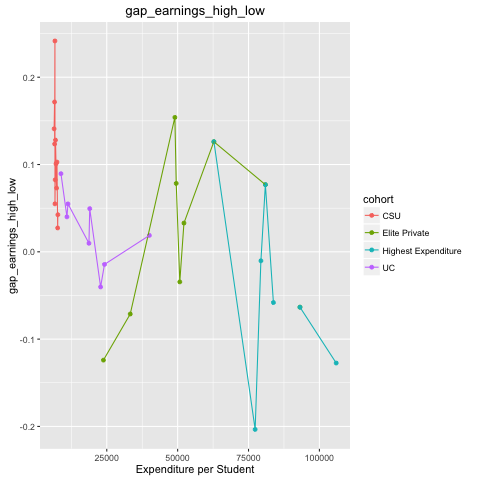
\includegraphics[width=0.3\textwidth]{../images/eda_scatterplots/gap_earnings_high_low_cohort.png}
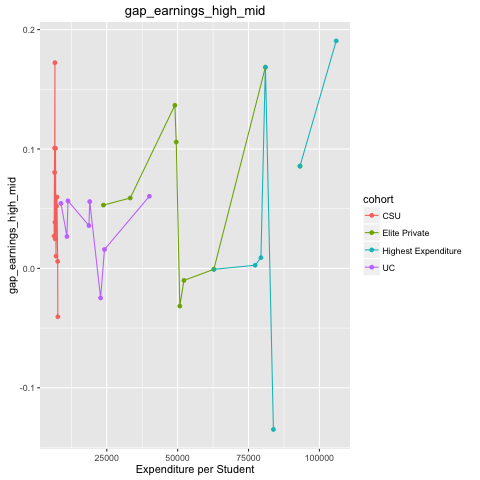
\includegraphics[width=0.3\textwidth]{../images/eda_scatterplots/gap_earnings_high_mid_cohort.png}
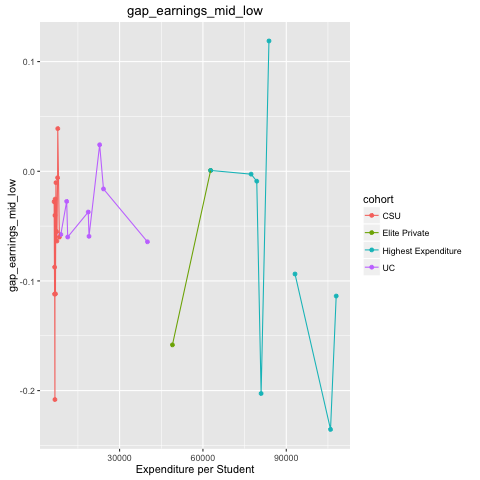
\includegraphics[width=0.3\textwidth]{../images/eda_scatterplots/gap_earnings_mid_low_cohort.png}
\caption{\label{fig:EarningsCohorts} We see a similar pattern with earnings. Interestingly, the data actually suggests that middle-income students do worse in comparison to high-income students as expenditures increase.}
\end{figure}


We now look at the full dataset to get a sense of the relationship across all schools in the US. We begin with completion rates.

\begin{figure}[H]
\centering
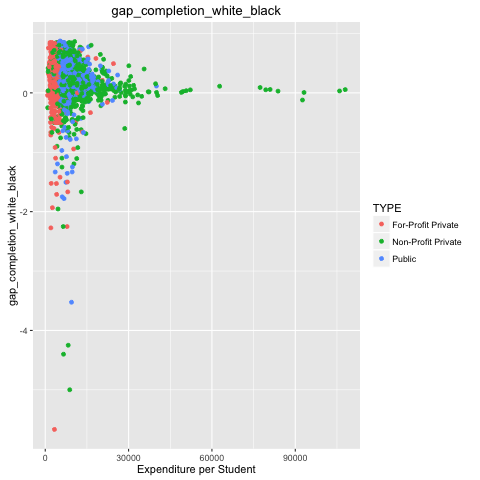
\includegraphics[width=0.3\textwidth]{../images/eda_scatterplots/gap_completion_white_black.png}
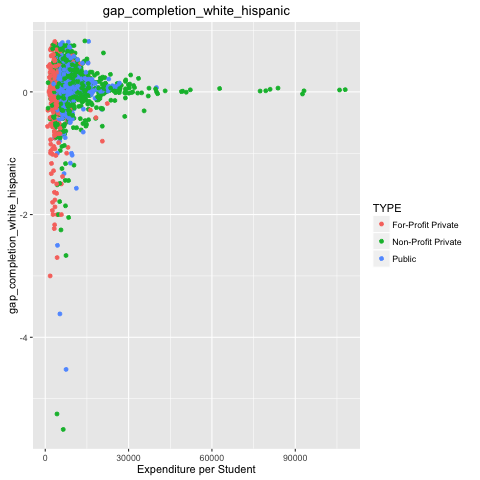
\includegraphics[width=0.3\textwidth]{../images/eda_scatterplots/gap_completion_white_hispanic.png}
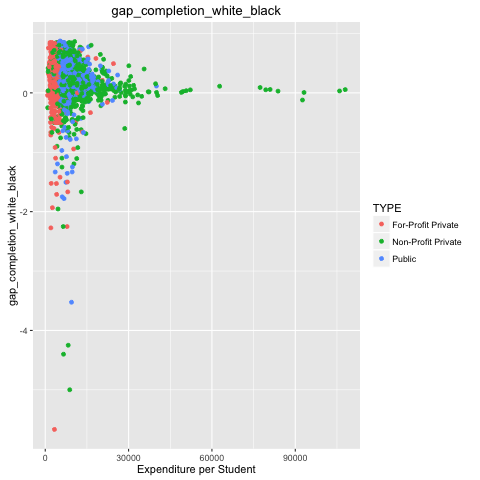
\includegraphics[width=0.3\textwidth]{../images/eda_scatterplots/gap_completion_white_black.png}
\caption{\label{fig:FullCompletionRates} While there are definite differences in expenditure by type of school, it is not obvious that achievement gaps decrease with expenditures. Generally, achievement gaps are not centered too far from zero, and there are quite a few outliers in both dimensions. However, it does look like variance decreases and outcome gaps cluster more closely around zero as expenditures increase.}
\end{figure}

We restrict our bounds to exclude the outliers to see if we can visually detect any patterns.

\begin{figure}[H]
\centering
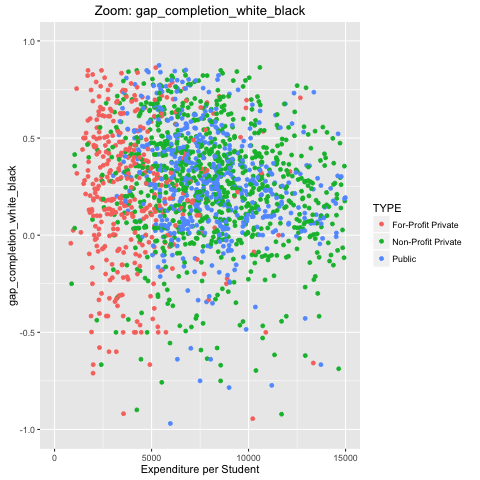
\includegraphics[width=0.3\textwidth]{../images/eda_scatterplots/gap_completion_white_black_zoom.png}
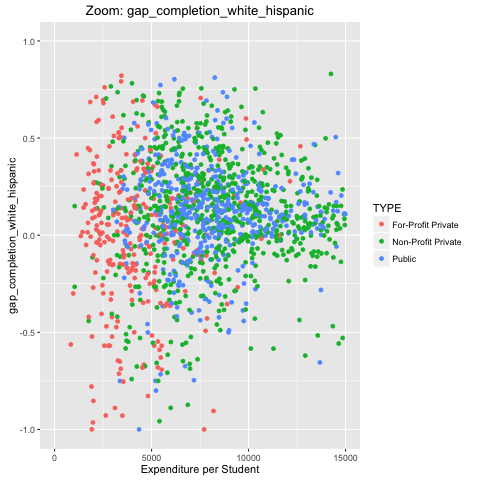
\includegraphics[width=0.3\textwidth]{../images/eda_scatterplots/gap_completion_white_hispanic_zoom.png}
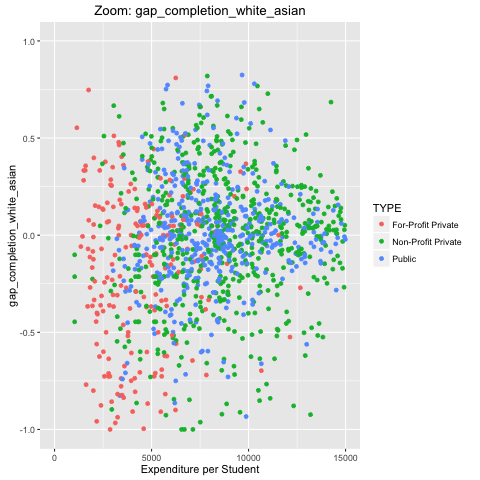
\includegraphics[width=0.3\textwidth]{../images/eda_scatterplots/gap_completion_white_asian_zoom.png}
\caption{\label{fig:ZoomCompletionRates} The data actually looks almost perfectly random.}
\end{figure}

Looking at our earnings metrics, we see a similar spread.

\begin{figure}[H]
\centering
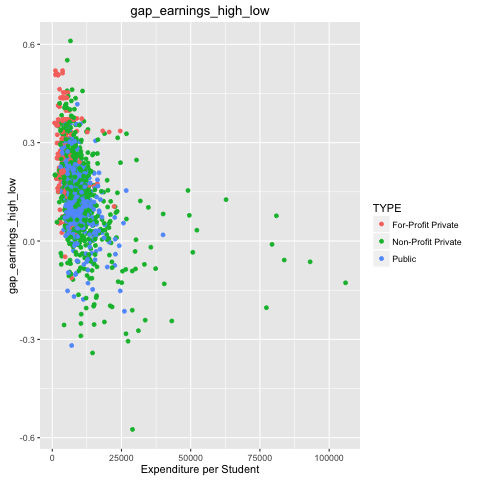
\includegraphics[width=0.3\textwidth]{../images/eda_scatterplots/gap_earnings_high_low.png}
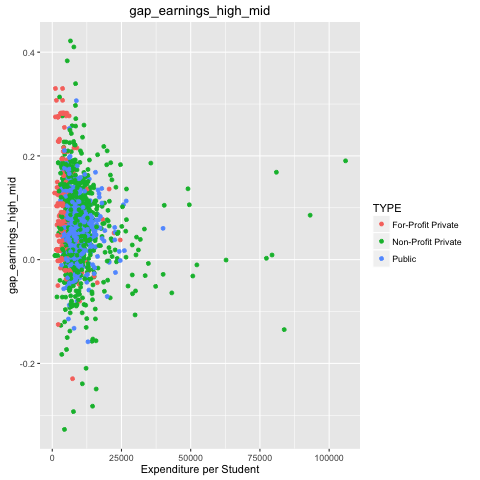
\includegraphics[width=0.3\textwidth]{../images/eda_scatterplots/gap_earnings_high_mid.png}
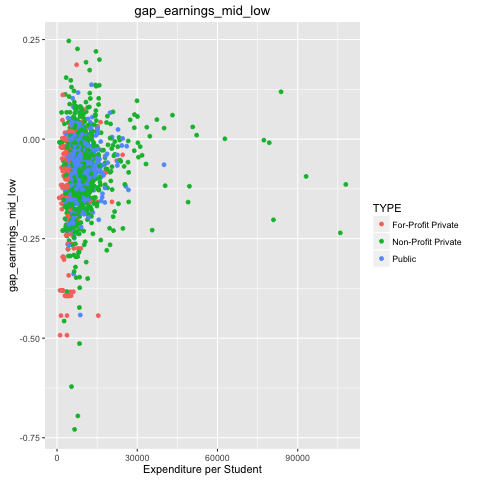
\includegraphics[width=0.3\textwidth]{../images/eda_scatterplots/gap_earnings_mid_low.png}
\caption{\label{fig:FullEarnings} We see a similar pattern, where variance decreases and the gap clusters closer to zero as expenditure increases. An interesting observation is that the gap between medium and low income terciles actually seems centered below zero - low income students on average seem to perform a bit better than their middle income peers.}
\end{figure}

However, restricting bounds produces a more interesting visual insight.

\begin{figure}[H]
\centering
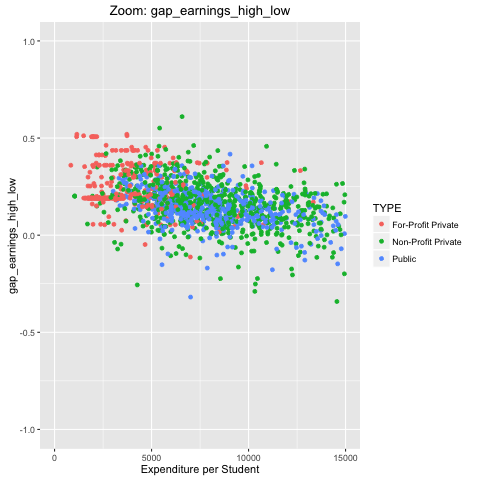
\includegraphics[width=0.3\textwidth]{../images/eda_scatterplots/gap_earnings_high_low_zoom.png}
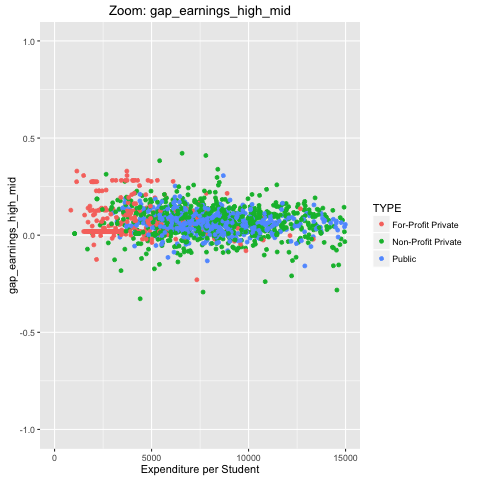
\includegraphics[width=0.3\textwidth]{../images/eda_scatterplots/gap_earnings_high_mid_zoom.png}
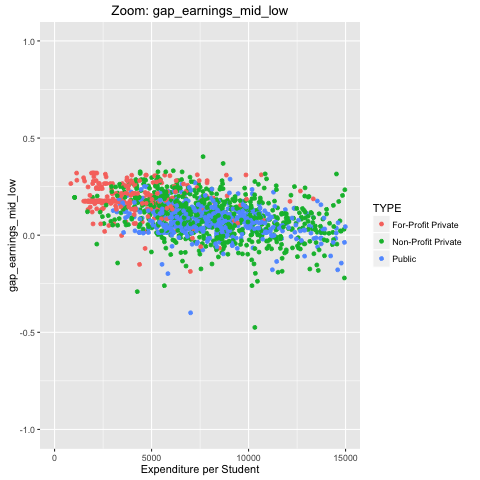
\includegraphics[width=0.3\textwidth]{../images/eda_scatterplots/gap_earnings_mid_low_zoom.png}
\caption{\label{fig:ZoomEarnings} Fascinatingly, we actually see a very clear negative correlation between expenditure and outcome gap for High-Low and High-Medium. Medium-Low seems to have no relationship.}
\end{figure}

The relationship between expenditure and outcome gap is not obvious, but there definitely seem to be some non-random patterns worth investigating. In the next sections, we undertake formal statistical analysis to develop more concrete conclusions about these patterns.


% !Rnw root = report.Rnw


\section{Anova Analysis on Type of School}

We want to first determine whether there is a significant outcome gap in terms of completion rate and earnings between the student groups at different types of institutions. Thus, we run an ANOVA model to assess whether there is a difference between public, private non-profit, and private school gap metrics. Let's first look at the analysis of variance of completion rates of black and white students.

% latex table generated in R 3.3.2 by xtable 1.8-2 package
% Sun Dec  4 20:24:55 2016
\begin{table}[ht]
\centering
\begin{tabular}{lrrrrr}
  \hline
 & Df & Sum Sq & Mean Sq & F value & Pr($>$F) \\ 
  \hline
cr\_w\_b\$CONTROL & 2 & 1.38 & 0.69 & 3.65 & 0.0261 \\ 
  Residuals      & 1938 & 366.44 & 0.19 &  &  \\ 
   \hline
\end{tabular}
\caption{ANOVA Table Completion Rate White and Black Students} 
\end{table}
As indicated by the high F statistics and low p-value, there is a significant difference between public, private non-profit, and private school black and white students completion rate gap metric. If we then look further for pair-wise comparisons in the Tukey Plot displayed, we see that the outcome gap is significant between Private For-Profit and Public schools, but not so much between Private For-Profit and Private Non-Profit or Private Non-Profit and Public schools.

\begin{figure}
\centering
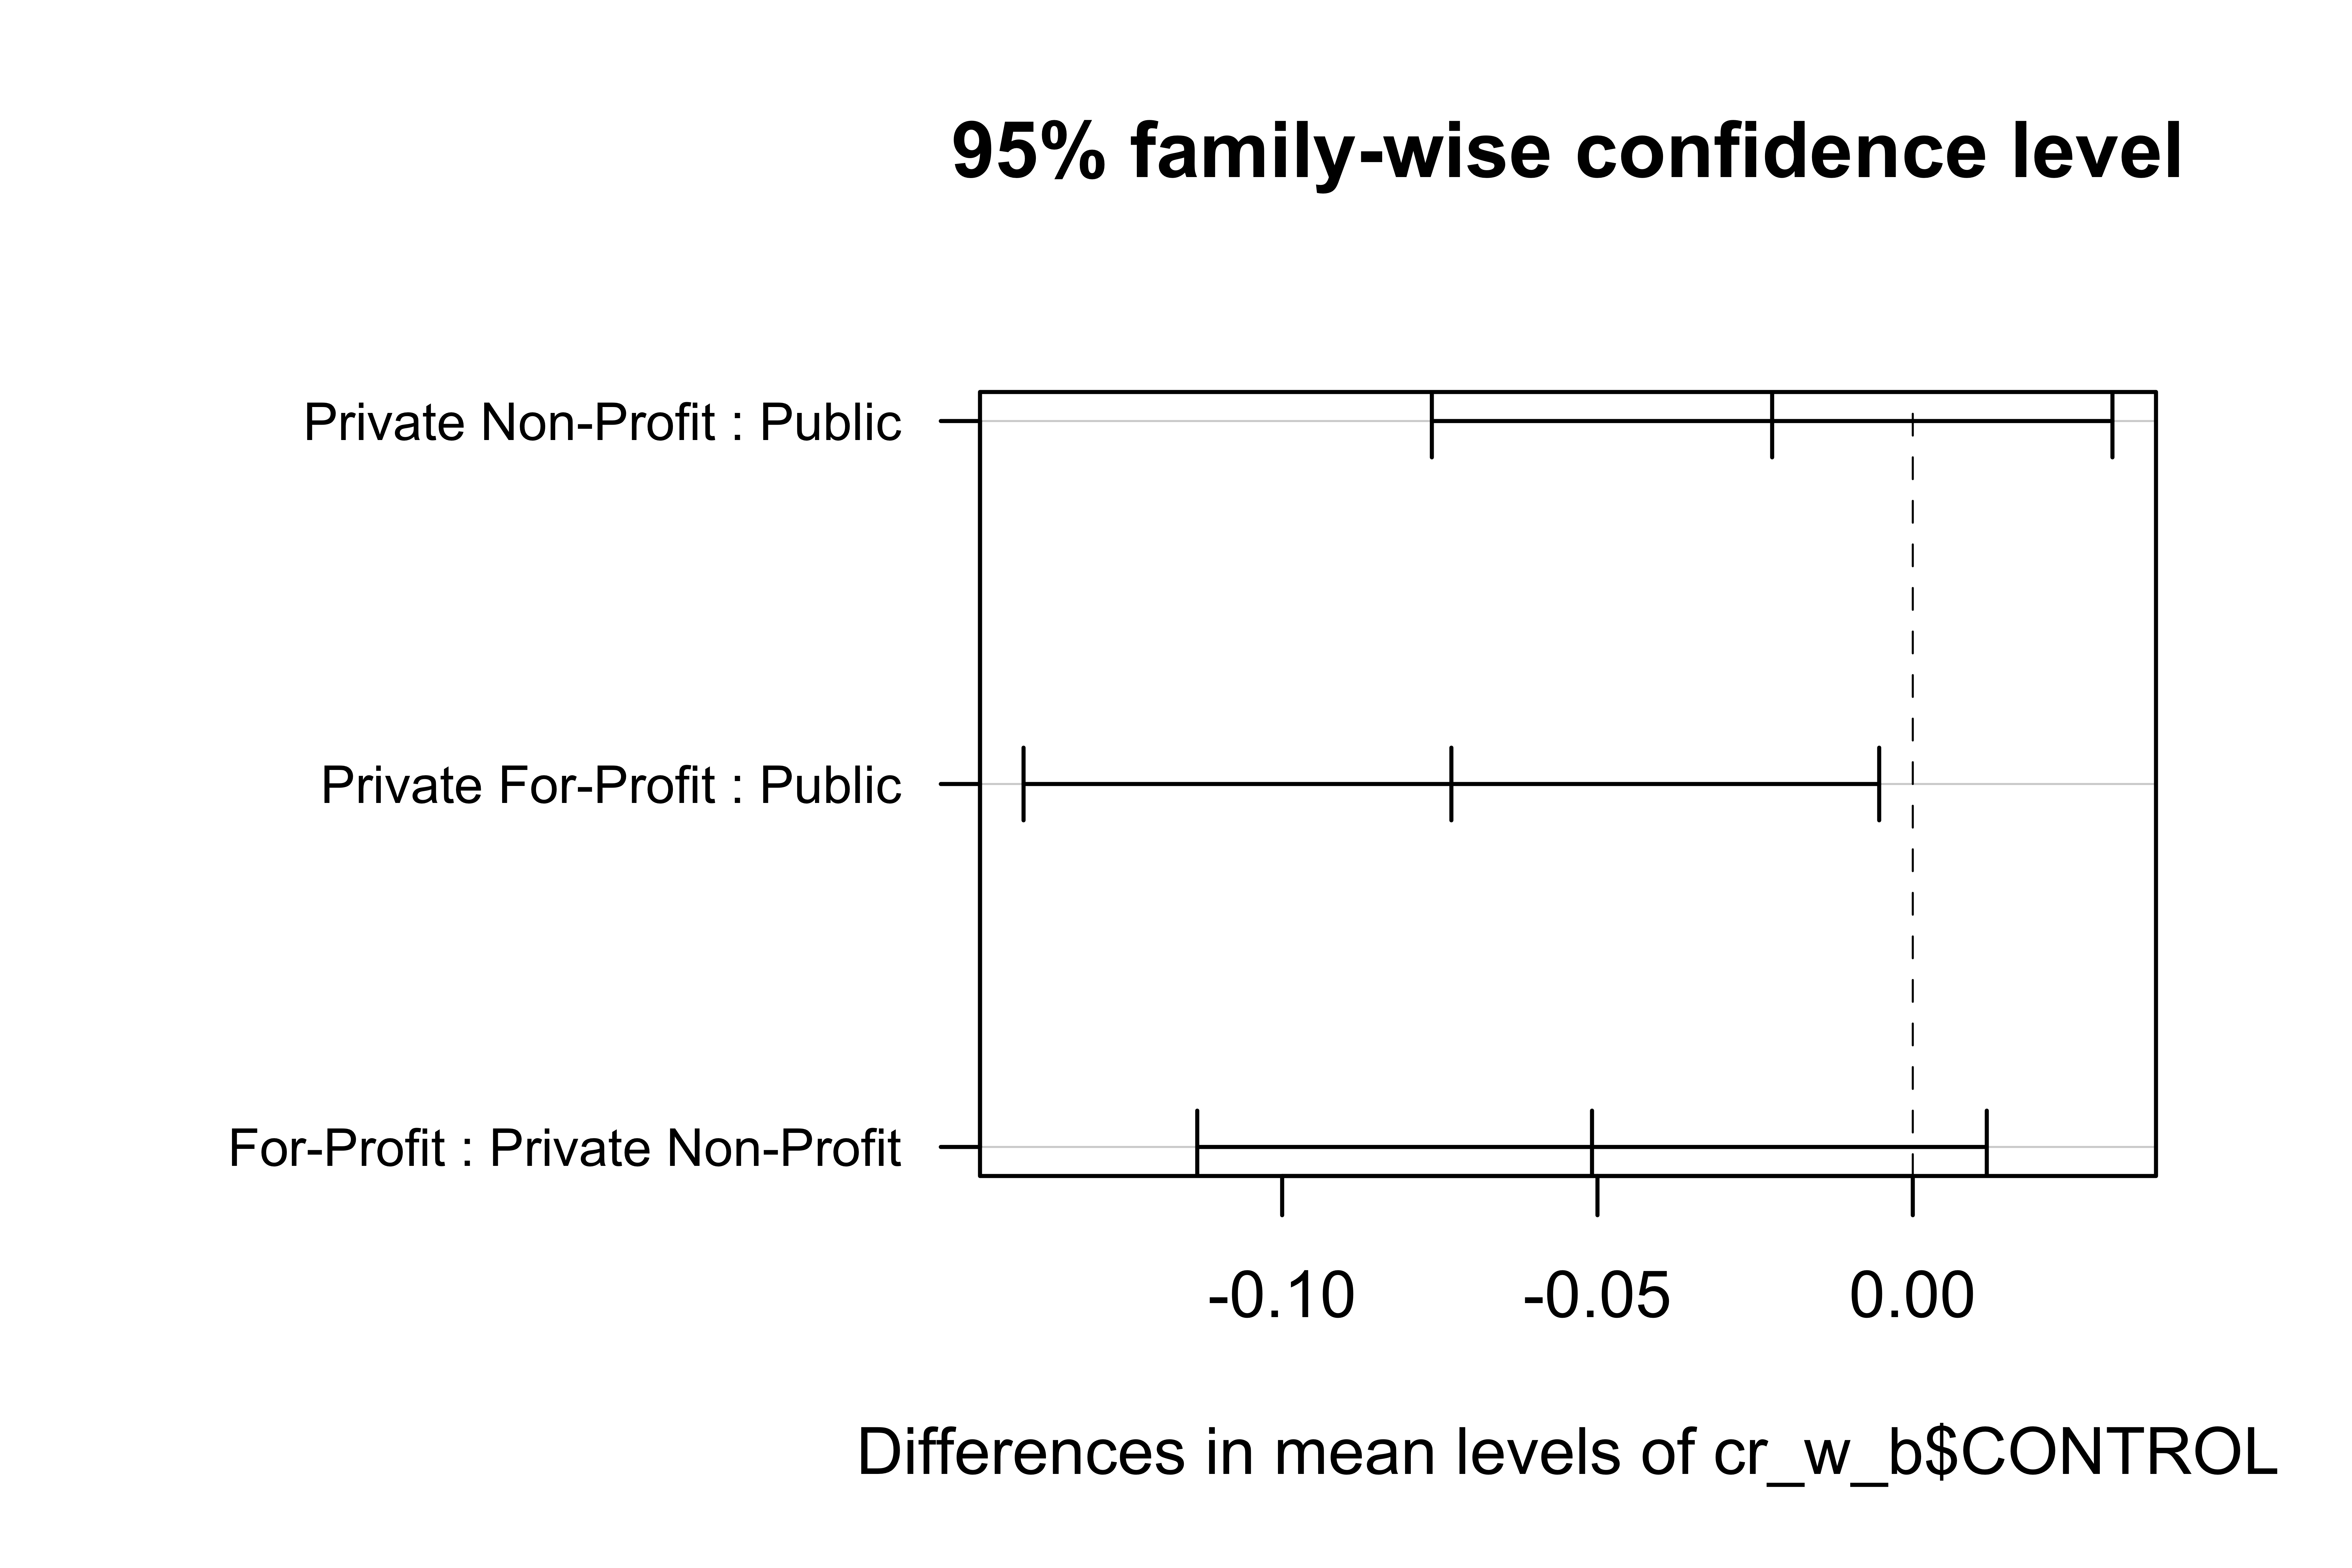
\includegraphics[width=0.8\textwidth]{../images/completion_rate_tukeyplot_white_black.png}
\caption{\label{fig:TukeyPlot}Tukey Plot Completion Rate White and Black Students}
\end{figure}

Doing similar analysis for completion rates by other racial groups, we see the completion rate gap metric is signifcant with Private For-Profit and Public schools in general. The gap metric is also signifcant with Private For-Profit and Private Non-Profit for Hispanic and White students.

\begin{table}[ht]
\centering
\begin{tabular}{rlrrr}
  \hline
 & Institutions & White\_Black & White\_Asian & White\_Hispanic \\ 
  \hline
1 & Private Non-Profit w/ Public & 0.54 & 0.63 & 0.82 \\ 
  2 & Private For-Profit w/ Public & 0.02 & 0.00 & 0.00 \\ 
  3 & Private For-Profit w/ Private Non-Profit & 0.11 & 0.00 & 0.00 \\ 
   \hline
\end{tabular}
\caption{Completion Rate P-Value Table} 
\end{table}
Looking at the earnings gap metric amongst different student income groups, we see that the outcome gap is signficant amongst all institution types for low income students. The gap is significant between Private Non-Profit and Public schools for high and mid income students.

\begin{table}[ht]
\centering
\begin{tabular}{rlrrr}
  \hline
 & Institutions & High\_Low & High\_Mid & Mid\_Low \\ 
  \hline
1 & Private Non-Profit w/ Public & 0.00 & 0.20 & 0.87 \\ 
  2 & Private For-Profit w/ Public & 0.00 & 0.30 & 0.01 \\ 
  3 & Private For-Profit w/ Private Non-Profit & 0.00 & 0.01 & 0.00 \\ 
   \hline
\end{tabular}
\caption{Earnings P-Value Table} 
\end{table}

\begin{figure}
\centering
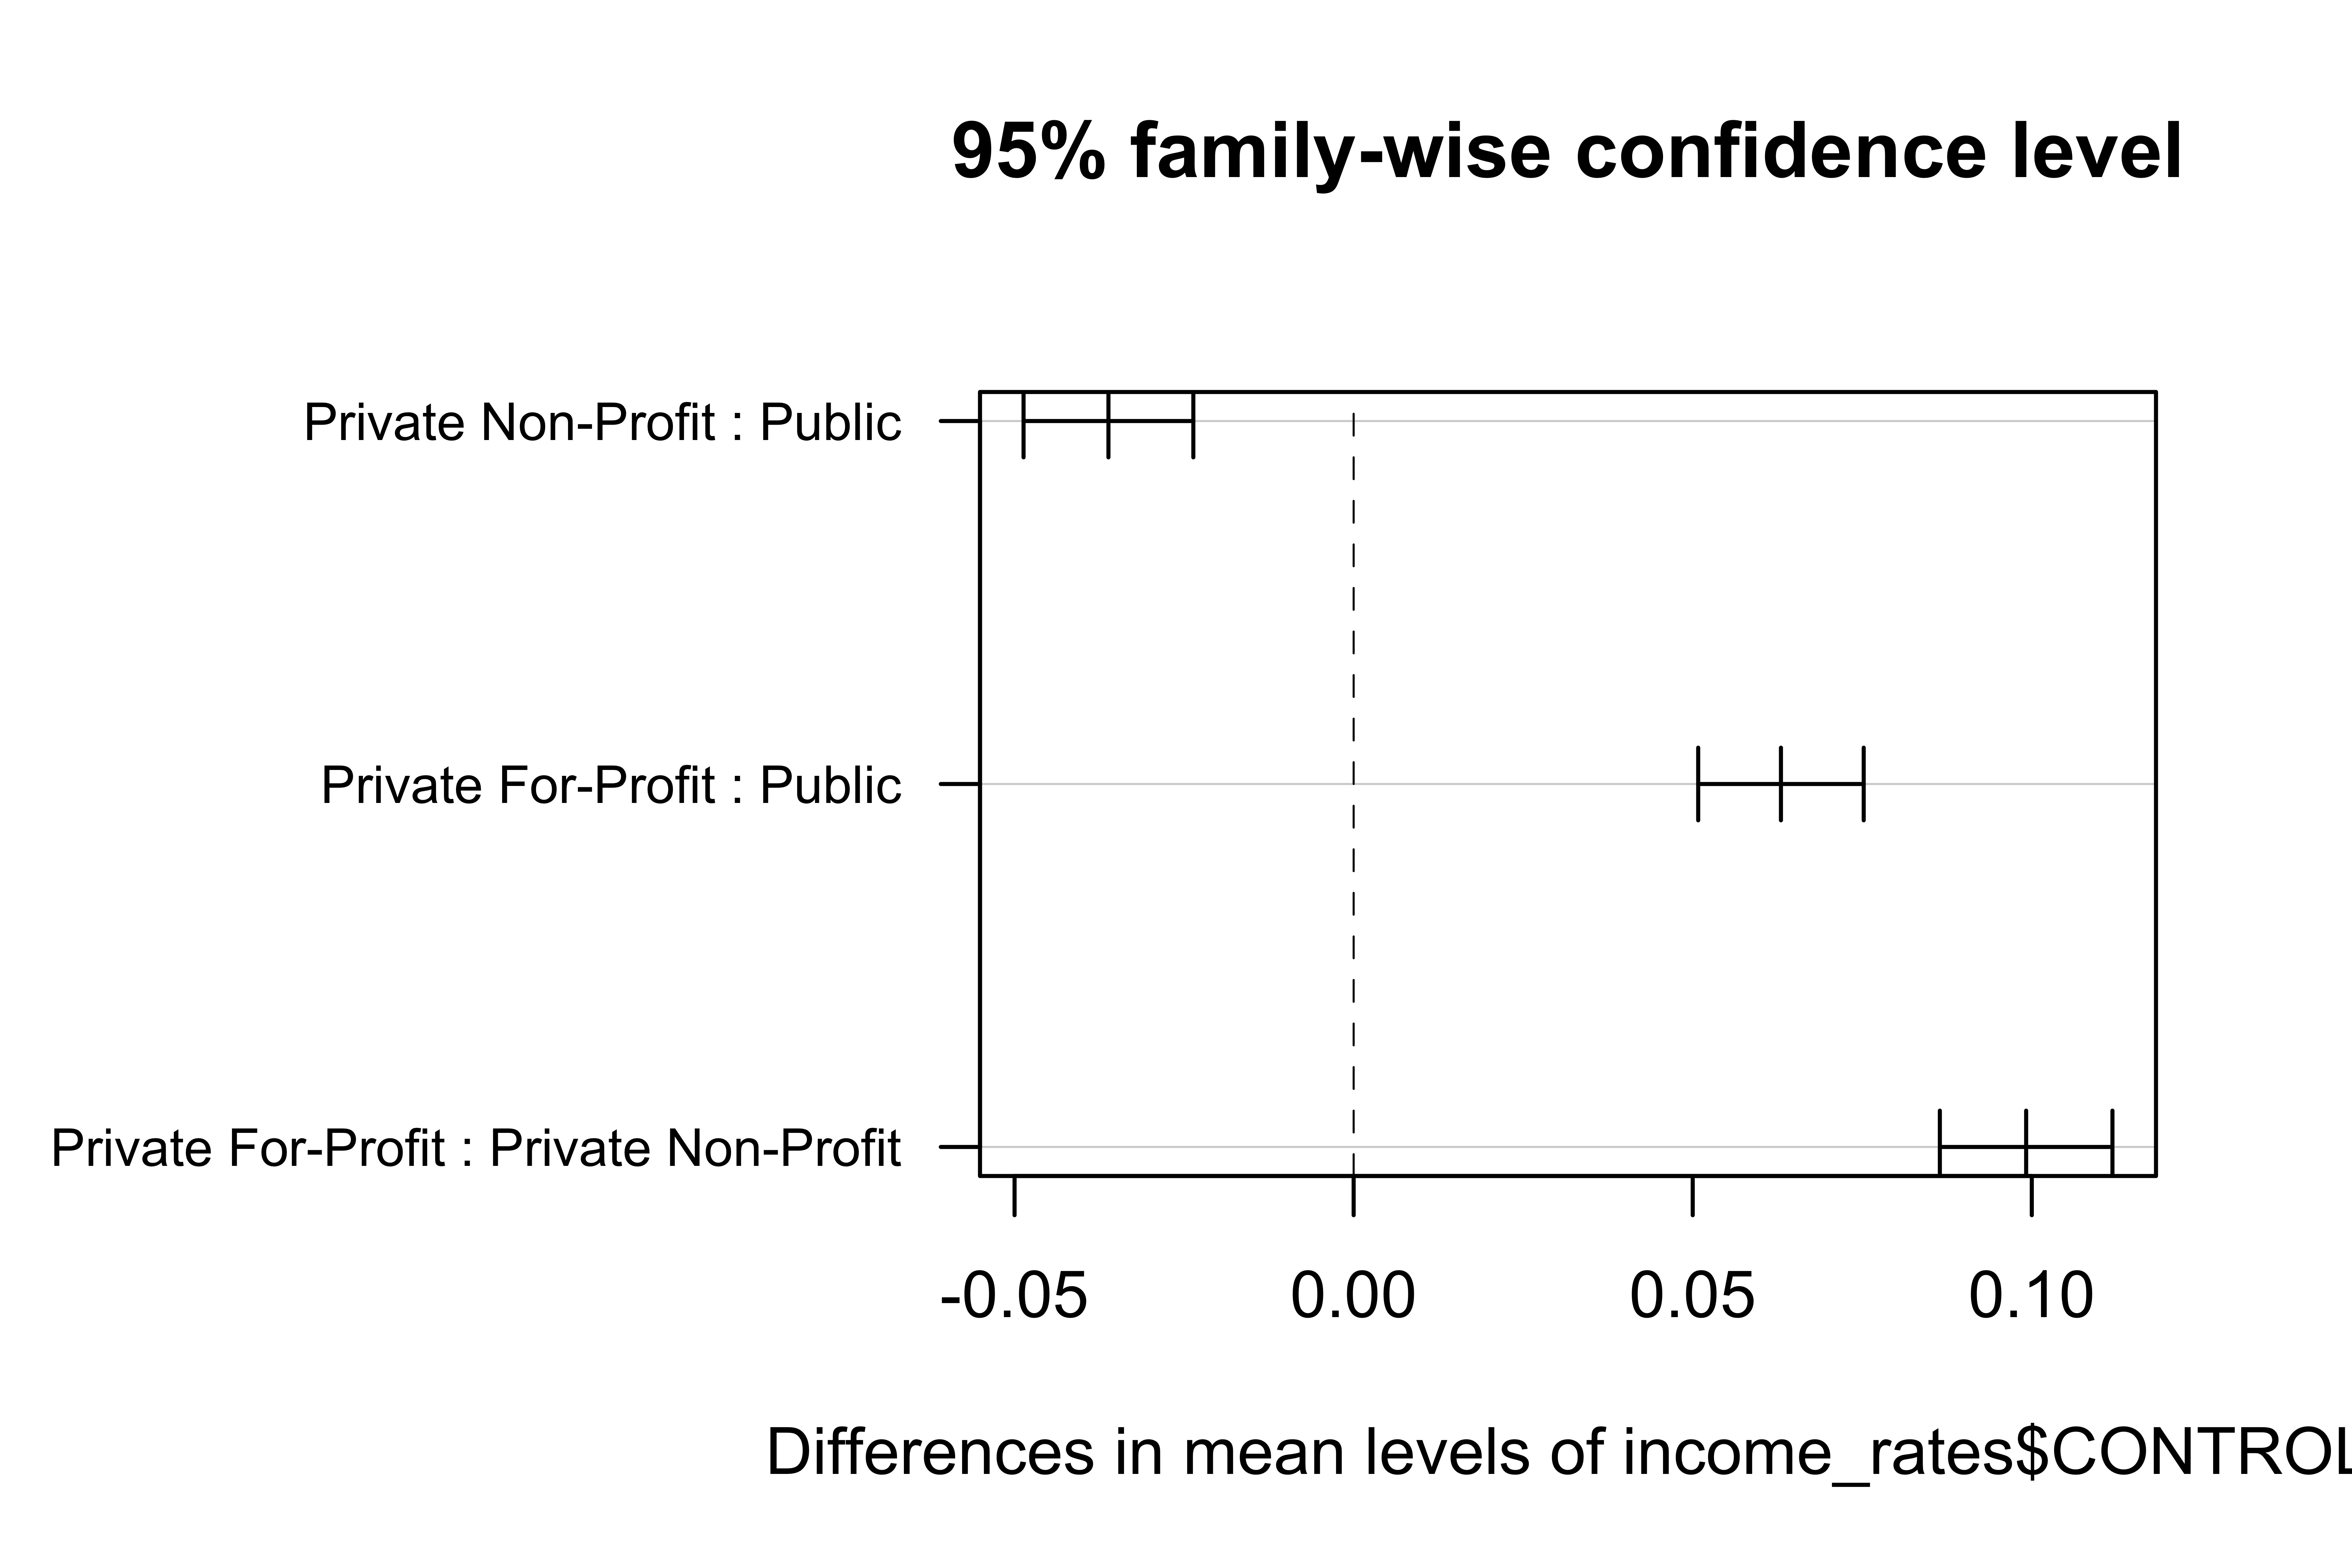
\includegraphics[width=0.8\textwidth]{../images/earnings_tukeyplot_high_low.png}
\caption{\label{fig:TukeyPlot2}Tukey Plot Earnings High and Low Income Students}
\end{figure}


% !Rnw root = report.Rnw

\section{Correlation Analysis on Expenditure per Student}

We are trying to find the relationship between the gap metrics, including the completion gap and income gap,  and school revenue per student, to see whether the school revenue per student has a negative correlation with the gap metrics. 

\subsection{Methodology}

We start our analysis by setting up null and alternative hypothesis. The null hypothesis is, $H_{0}$, that there is no relationship between gap metrics and school revenue per student; the alternative hypothesis is, $H_{1}$, that there is a relationship between gap metrics and school revenue per student. These are equal to the following that $H_{0}: \beta_1 = 0$ and $H_{0}: \beta_1 \neg 0$. To test the hypothesis, we apply a simple regression model like $Gapterms= \beta_0 + \beta_1 TUITFTE$. For both completion gap and income gap, we have three pairs of groups due to three race groups we have, thus we also have three regressions for each gap metric. In this case, we will use the least squares model on our data for the regression analysis. 

Before we apply the simple model, we do some graphs to see whether the data shows a linear relationship or not. If they do not appear a linear relationship, we do some data processing like log transformation to make the data normally distributed. 

For completion gap, the linear model gives an almost straight fitted line, thus we are using a simple linear model between completion gap and TUITFTE; while for income gap, it turns out that it is better to use a linear-log model for this data set. Bellow shows the scatter plots with fitted lines of each model chosen.


\subsection{Results}

Running regression through R, we can compute get the estimated coefficients. The regression coefficients for completion gap is given in the tables below:


\begin{table}[ht]
\centering
\caption{Information about Regression Coefficents of white and asian} 
\begin{tabular}{rrrrr}
  \hline
 & Estimate & Std. Error & t value & Pr($>$$|$t$|$) \\ 
  \hline
(Intercept) & -0.16 & 0.03 & -5.17 & 0.00 \\ 
  TUTFTE & 0.00 & 0.00 & 1.07 & 0.28 \\ 
   \hline
\end{tabular}
\end{table}
\begin{table}[ht]
\centering
\caption{Information about Regression Coefficents of white and black} 
\begin{tabular}{rrrrr}
  \hline
 & Estimate & Std. Error & t value & Pr($>$$|$t$|$) \\ 
  \hline
(Intercept) & 0.28 & 0.02 & 13.40 & 0.00 \\ 
  TUTFTE & -0.00 & 0.00 & -4.27 & 0.00 \\ 
   \hline
\end{tabular}
\end{table}
\begin{table}[ht]
\centering
\caption{Information about Regression Coefficents of white and hispanic} 
\begin{tabular}{rrrrr}
  \hline
 & Estimate & Std. Error & t value & Pr($>$$|$t$|$) \\ 
  \hline
(Intercept) & 0.04 & 0.03 & 1.71 & 0.09 \\ 
  TUTFTE & -0.00 & 0.00 & -1.07 & 0.28 \\ 
   \hline
\end{tabular}
\end{table}
More information about the least squares model from the regression analysis is given in the table below:

\begin{table}[ht]
\centering
\caption{Regression Quality Indices} 
\begin{tabular}{rlr}
  \hline
 & Quantity & Value \\ 
  \hline
1 & RSSwa & 0.59 \\ 
  2 & R2wa & 0.00 \\ 
  3 & F-statwa & 1.15 \\ 
  4 & RSSwb & 0.43 \\ 
  5 & R2wb & 0.01 \\ 
  6 & F-statwb & 18.20 \\ 
  7 & RSSwc & 0.51 \\ 
  8 & R2wc & 0.00 \\ 
  9 & F-statwc & 1.15 \\ 
   \hline
\end{tabular}
\end{table}
OLS regression summary statistics shows that there is statistically significant relationship between completion gap between white and asian and that between white and hispanic with school revenue per student. However, the completion gap between white and black has a statistically significant negative relationship with the school revenue per student and also has a really high F-statistics `r   `, while this model has a quite low R-squared value with `r `,  showing that we omits other necessary factors in this analysis. 


\begin{table}[ht]
\centering
\caption{Information about Regression Coefficents of high and low} 
\begin{tabular}{rrrrr}
  \hline
 & Estimate & Std. Error & t value & Pr($>$$|$t$|$) \\ 
  \hline
(Intercept) & 0.49 & 0.03 & 19.34 & 0.00 \\ 
  TUITFTE & -0.03 & 0.00 & -12.05 & 0.00 \\ 
   \hline
\end{tabular}
\end{table}
\begin{table}[ht]
\centering
\caption{Information about Regression Coefficents of high and middle} 
\begin{tabular}{rrrrr}
  \hline
 & Estimate & Std. Error & t value & Pr($>$$|$t$|$) \\ 
  \hline
(Intercept) & 0.21 & 0.02 & 12.85 & 0.00 \\ 
  TUITFTE & -0.02 & 0.00 & -8.47 & 0.00 \\ 
   \hline
\end{tabular}
\end{table}
\begin{table}[ht]
\centering
\caption{Information about Regression Coefficents of middle and low} 
\begin{tabular}{rrrrr}
  \hline
 & Estimate & Std. Error & t value & Pr($>$$|$t$|$) \\ 
  \hline
(Intercept) & -0.24 & 0.02 & -12.04 & 0.00 \\ 
  TUITFTE & 0.02 & 0.00 & 7.72 & 0.00 \\ 
   \hline
\end{tabular}
\end{table}
More information about the least squares model from the regression analysis is given in the table below:

\begin{table}[ht]
\centering
\caption{Regression Quality Indices} 
\begin{tabular}{rlr}
  \hline
 & Quantity2 & Value2 \\ 
  \hline
1 & RSShl & 0.13 \\ 
  2 & R2hl & 0.04 \\ 
  3 & F-stathl & 145.10 \\ 
  4 & RSShm & 0.08 \\ 
  5 & R2hm & 0.02 \\ 
  6 & F-stathm & 71.68 \\ 
  7 & RSSml & 0.10 \\ 
  8 & R2ml & 0.02 \\ 
  9 & F-statml & 59.52 \\ 
   \hline
\end{tabular}
\end{table}
OLS regression summary statistics shows that there is statistically significant negative relationship between income gap and the school revenue per student for each pair of income group, including high-low, high-middle and middle-low. To be noticed that all three regressions have very high F-statistics: `r `, showing reliability, while low R-squared value. This is reasonable that we here only have a very simple model. Additionally, we are using linear-log model for income gap, thus one percentage change in school revenue per student would result in unit change in income gap. 


The above regressions shows that there do exist a negative relationship between completion rates gap and income gap of different race groups with the school revenue per student. Then, we would like to make a data-based argument that increasing funding for public schools can decrease the gap metric. To do this, we will model the gap metrics as a function of school revenue split by public and private schools. In other words, we first split the dataset by type of school, including public and private, and then run a linear model: $Gapterms= \beta_0 + \beta_1 INEXPFTE$, and then compare slopes and intercepts between public and private schools. INEXPFTE stands for  instructional expenditures per full-time student. 


\begin{table}[ht]
\centering
\caption{Completion Gap Interception comparsion} 
\begin{tabular}{rlr}
  \hline
 & Quantity3 & Value3 \\ 
  \hline
1 & PublicwaIntc & -0.13 \\ 
  2 & PrivatewaIntc & -0.27 \\ 
  3 & PublicwbIntc & 0.32 \\ 
  4 & PrivatewbIntc & 0.22 \\ 
  5 & PublicwhIntc & 0.01 \\ 
  6 & PrivatewhIntc & -0.03 \\ 
   \hline
\end{tabular}
\end{table}
\begin{table}[ht]
\centering
\caption{Completion Gap Slope comparsion} 
\begin{tabular}{rlr}
  \hline
 & Quantity4 & Value4 \\ 
  \hline
public\_school\_wa\$INEXPFTE & PublicwaIntc & 0.00 \\ 
  private\_school\_wa\$INEXPFTE & PrivatewaIntc & 0.00 \\ 
  public\_school\_wb\$INEXPFTE & PublicwbIntc & -0.00 \\ 
  private\_school\_wb\$INEXPFTE & PrivatewbIntc & -0.00 \\ 
  public\_school\_wh\$INEXPFTE & PublicwhIntc & 0.00 \\ 
  private\_school\_wh\$INEXPFTE & PrivatewhIntc & 0.00 \\ 
   \hline
\end{tabular}
\end{table}
\begin{table}[ht]
\centering
\caption{Income Gap Interception comparsion} 
\begin{tabular}{rlr}
  \hline
 & Quantity5 & Value5 \\ 
  \hline
1 & PublichlIntc & 0.25 \\ 
  2 & PrivatehlIntc & 0.24 \\ 
  3 & PublichmIntc & 0.10 \\ 
  4 & PrivatehmIntc & 0.08 \\ 
  5 & PublicmlIntc & -0.11 \\ 
  6 & PrivatemlIntc & -0.09 \\ 
   \hline
\end{tabular}
\end{table}
\begin{table}[ht]
\centering
\caption{Income Gap Slope comparsion} 
\begin{tabular}{rlr}
  \hline
 & Quantity6 & Value6 \\ 
  \hline
1 & PublichlIntc & -0.00 \\ 
  2 & PrivatehlIntc & -0.00 \\ 
  3 & PublichmIntc & -0.00 \\ 
  4 & PrivatehmIntc & -0.00 \\ 
  5 & PublicmlIntc & 0.00 \\ 
  6 & PrivatemlIntc & 0.00 \\ 
   \hline
\end{tabular}
\end{table}
For completion rate gap, the private school turns to have smaller interception in three pairs of race groups. This proves our argument that private schools, which often have more funding for instruction, have a smaller completion rate gap. Similarily, for income gap, the private school also shows better standing in the interception in three pairs of income groups. However, for slopes, white-asian group has a bigger slope, while white-black group has a less steep slope, which might imply that increasing in instruction funding would lead to reduction in completion rate gap, while the efficiency depending on the race group. For income gap, we can also see that higher efficiency in high-lower group. 

I also ran regressions for nonprofit private schools and profit private schools.......................Further proves our argument...........

Summary of second model:
1. Negative relationship between gap metrics and school revenue.
2. More school funding, smaller gap. 


\newpage


% !Rnw root = report.Rnw
\newpage
\section{Random Forest}

Our goal in this section is to do some inference on other possible predictors. We identified fourteen variables which we considered possibly relevant and briefly summarize them in Table 16.
  

 
\begin{table}[ht]
\centering
\caption{Description of Random Forest Explanatory Variables} 
\begin{tabular}{rll}
  \hline
 & Explanatory.Variable & Description \\ 
  \hline
1 & SCH\_DEG & Highest Degree Awarded \\ 
  2 & PREDDEG & Predominant Degree Awarded \\ 
  3 & REGION & Region of the US \\ 
  4 & LOCALE & Locale type (e.g. Urban = 12) \\ 
  5 & ADM\_RATE & Admission Rate \\ 
  6 & UGDS\_WHITE & White Proportion of Student Body \\ 
  7 & UGDS\_BLACK & Black Proportion of Student Body \\ 
  8 & UGDS\_HISP & Hispanic Proportion of Student Body \\ 
  9 & UGDS\_ASIAN & Asian Proportion of Student Body \\ 
  10 & COSTT4\_A & Average Cost to Attend \\ 
  11 & MEDIAN\_HH\_INC & Median Household Income \\ 
  12 & POVERTY\_RATE & Poverty Rate of Students \\ 
  13 & INEXPFTE & Expenditures per Student \\ 
  14 & CONTROL & Institution Type \\ 
   \hline
\end{tabular}
\end{table}

For each gap metric, we ran a random forest regression on the 14 variables, with 100 trees per forest. We checked the error plots to verify that we had reached a plateau in error at this number of trees. We also tried a few values for the number of variables to consider at each split, and got the best performance with 4.

\begin{figure}[H]
\centering
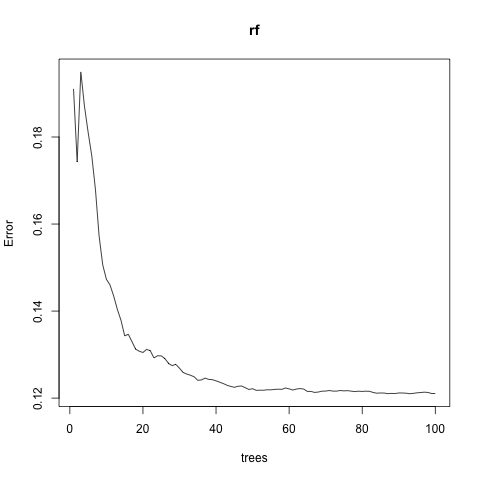
\includegraphics[width=0.5\textwidth]{../images/rf_treesgap_completion_white_black.png}
\caption{\label{fig: WBRFerror} We see that increasing the number of trees is unlikely to produce better results.}
\end{figure}

In this situation, we are not attempting to build a predictive model. We are focused on identifying interesting relationships. Still, our models performed fairly poorly in terms of percent variance explained, so we should take these results with a grain of salt.

\begin{figure}[H]
\centering
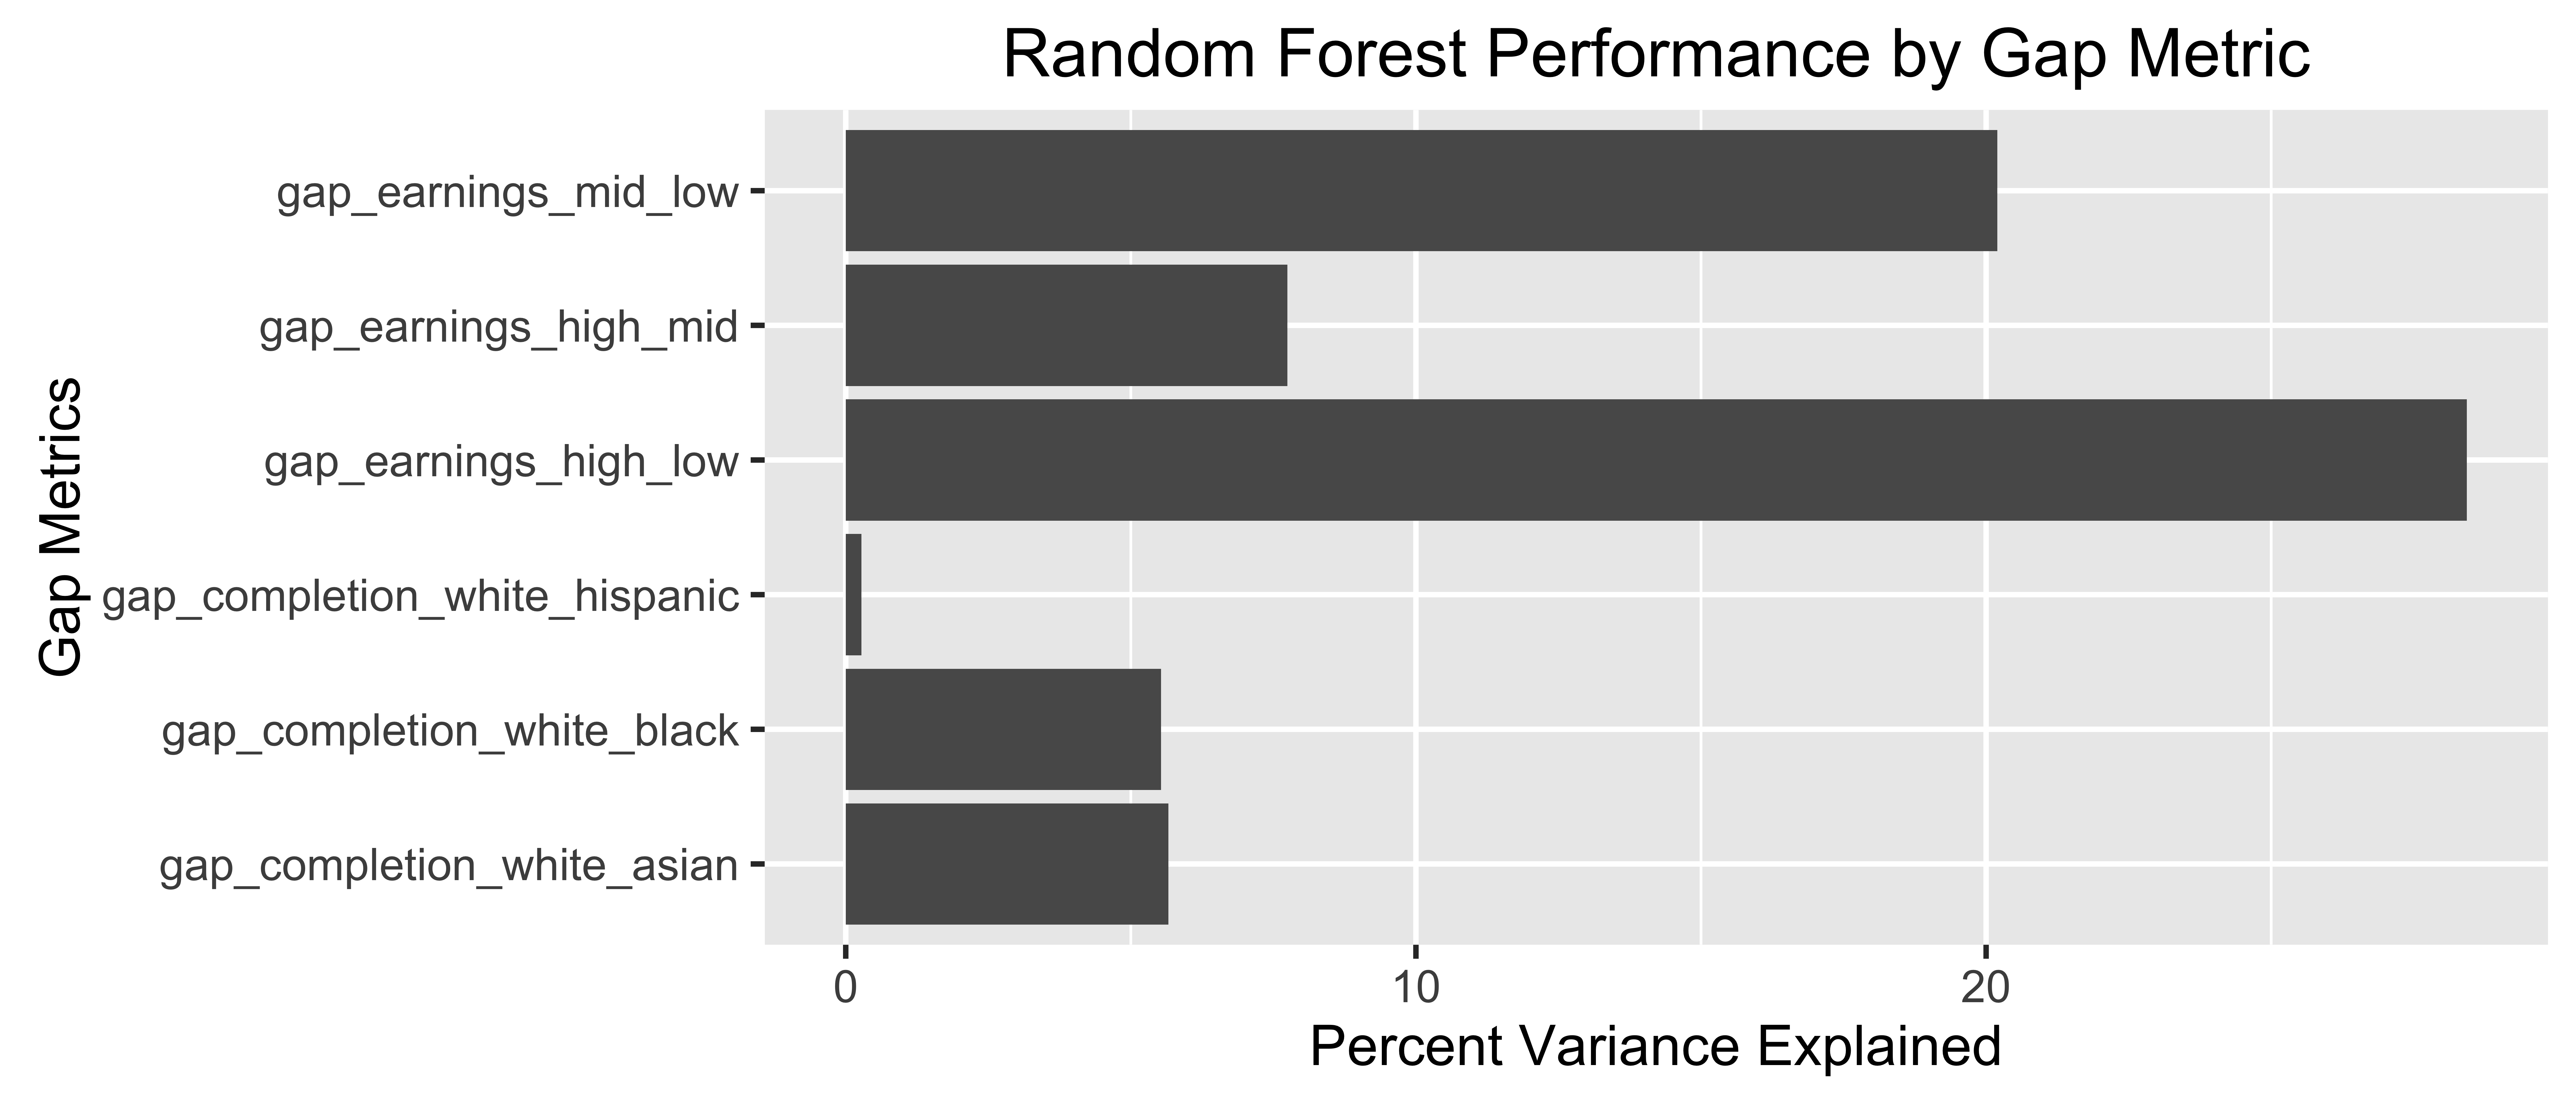
\includegraphics[width=0.5\textwidth]{../images/rf_performance.png}
\caption{\label{fig: RFPerforomance} Most of our Random Forests performed extremely poorly. The best model was that which explained the variance between High and Low Income terciles. Interestingly, this recalls that the most visually noticeable trend in EDA was between these groups.}
\end{figure}

The reason we chose random forest was that this model provides a heuristic for variable importance. This statistic is the result of caculating the average increase in node purity associated with each variable over all one hundred trees. This metric is difficult to understand without some conception of how a decision tree is constructed, but an abstract explanation is that the statistic indicates how much more accurate a tree is in predicting the target when given the variable. Therefore, a comparison of node purity increase across the variables for the separate models can provide some insight for our purposes.

Because the spread of the completion rate gaps was much larger than the spread of earning gaps, we consider these types separately.


\begin{figure}[H]
\centering
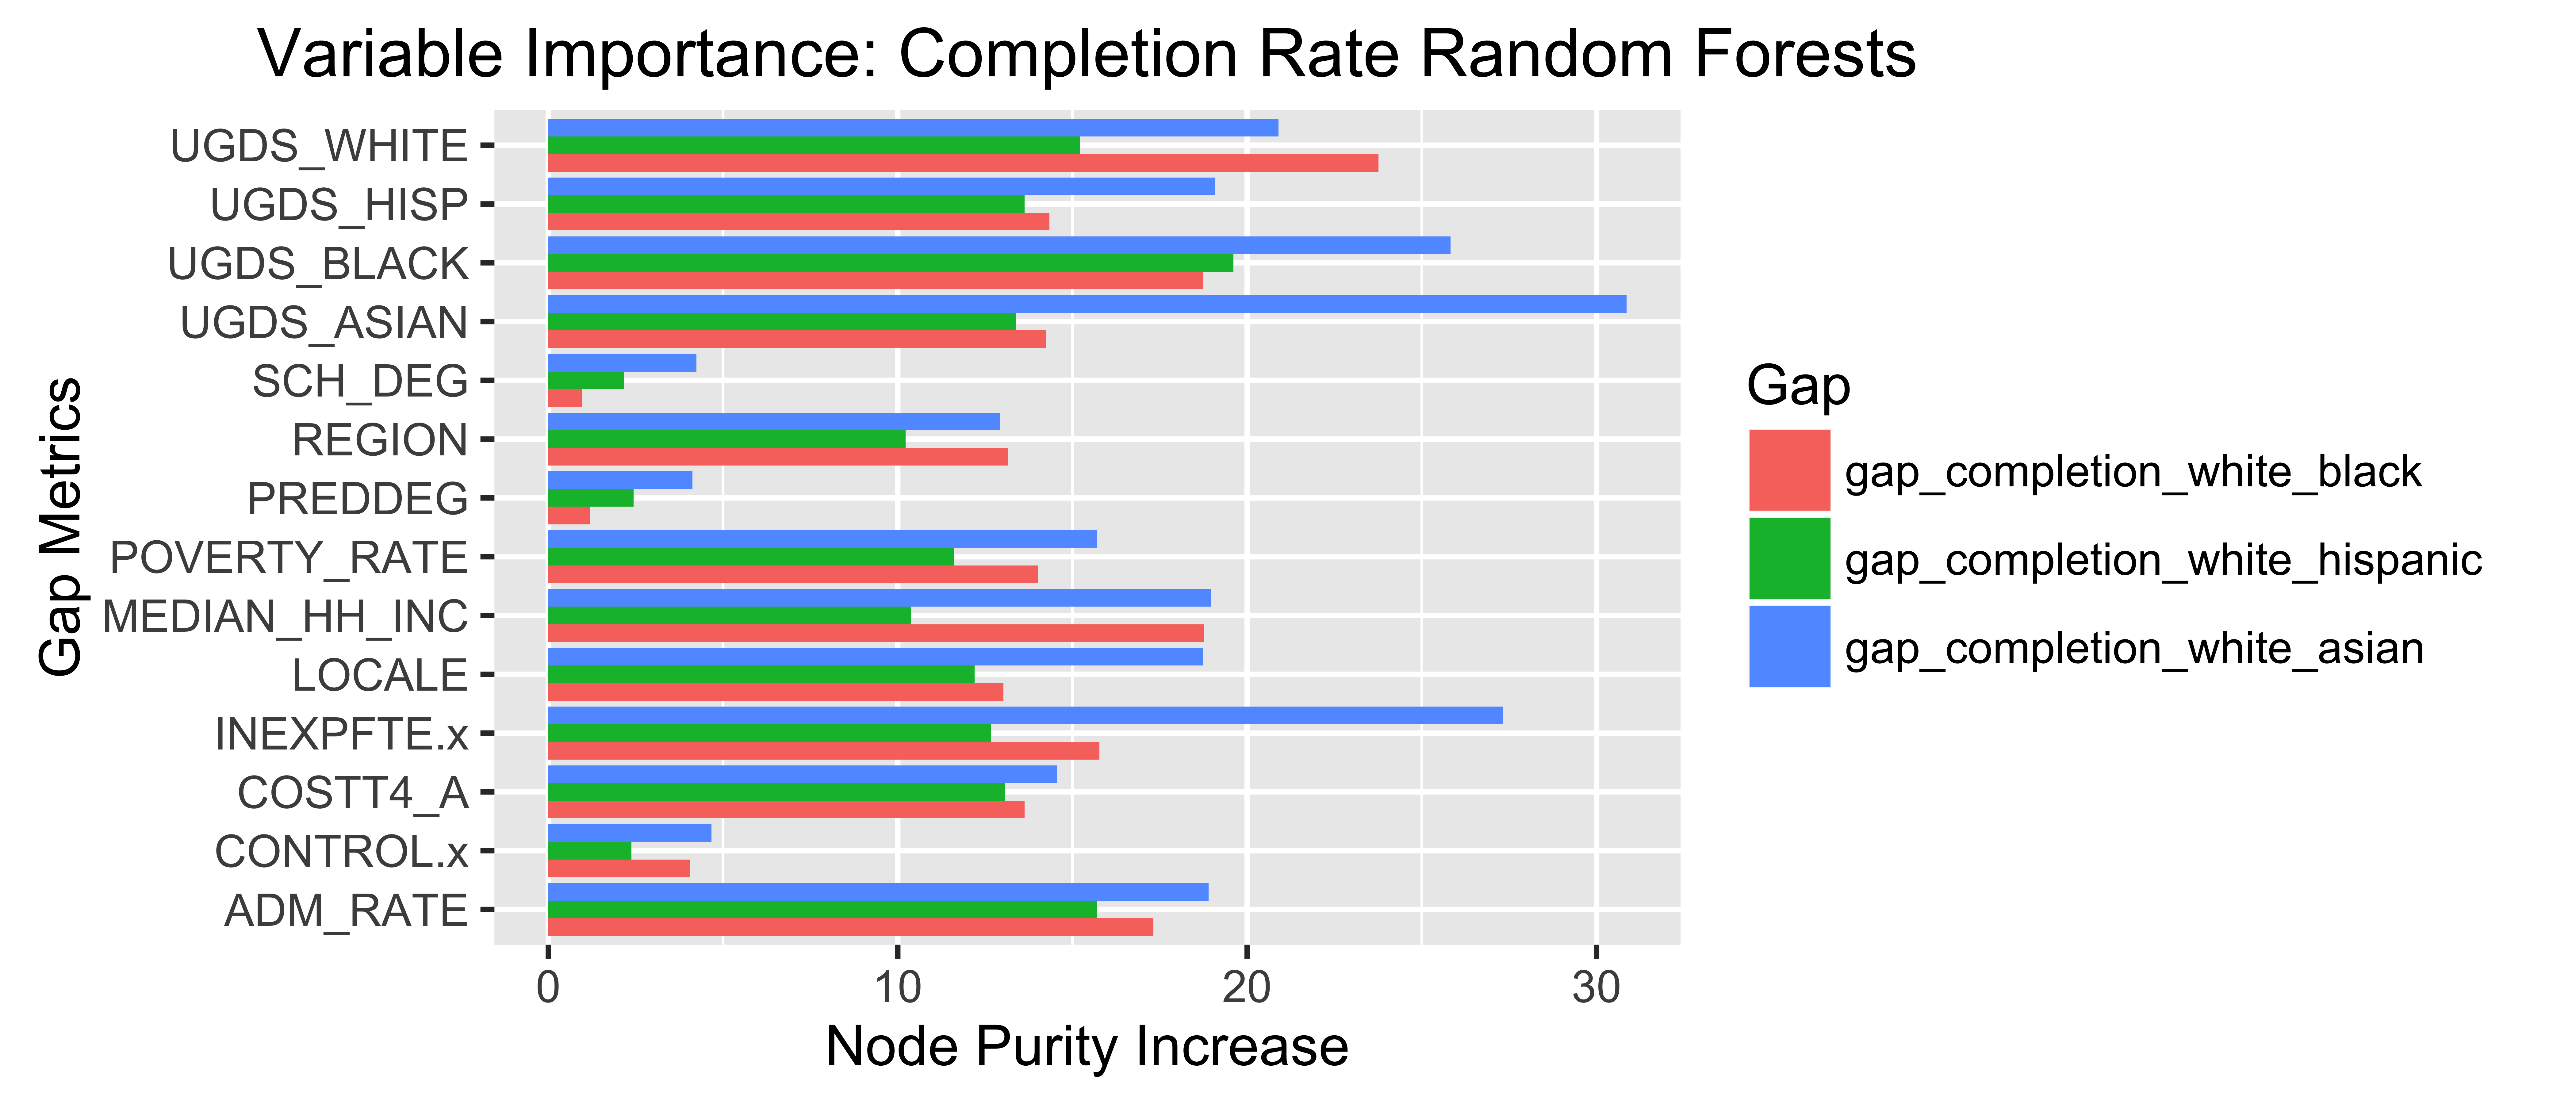
\includegraphics[width=0.5\textwidth]{../images/rf_importance_completion.png}
\caption{\label{fig: RFCompletionRates} The most notable takeaway is that INEXPFTE is in fact one of the most important predictors, especially for the white Asian gap. Recall that this model performed the best of the completion rate models. Another noticeable trend is that the proportion of the student body which is Asian is a strong predictor for the white Asian completion gap. We also see a similar trend with the UGDSBlack for the white black completion gap. Generally, the diversity of the student body seems to be fairly relevant.}
\end{figure}


\begin{figure}[H]
\centering
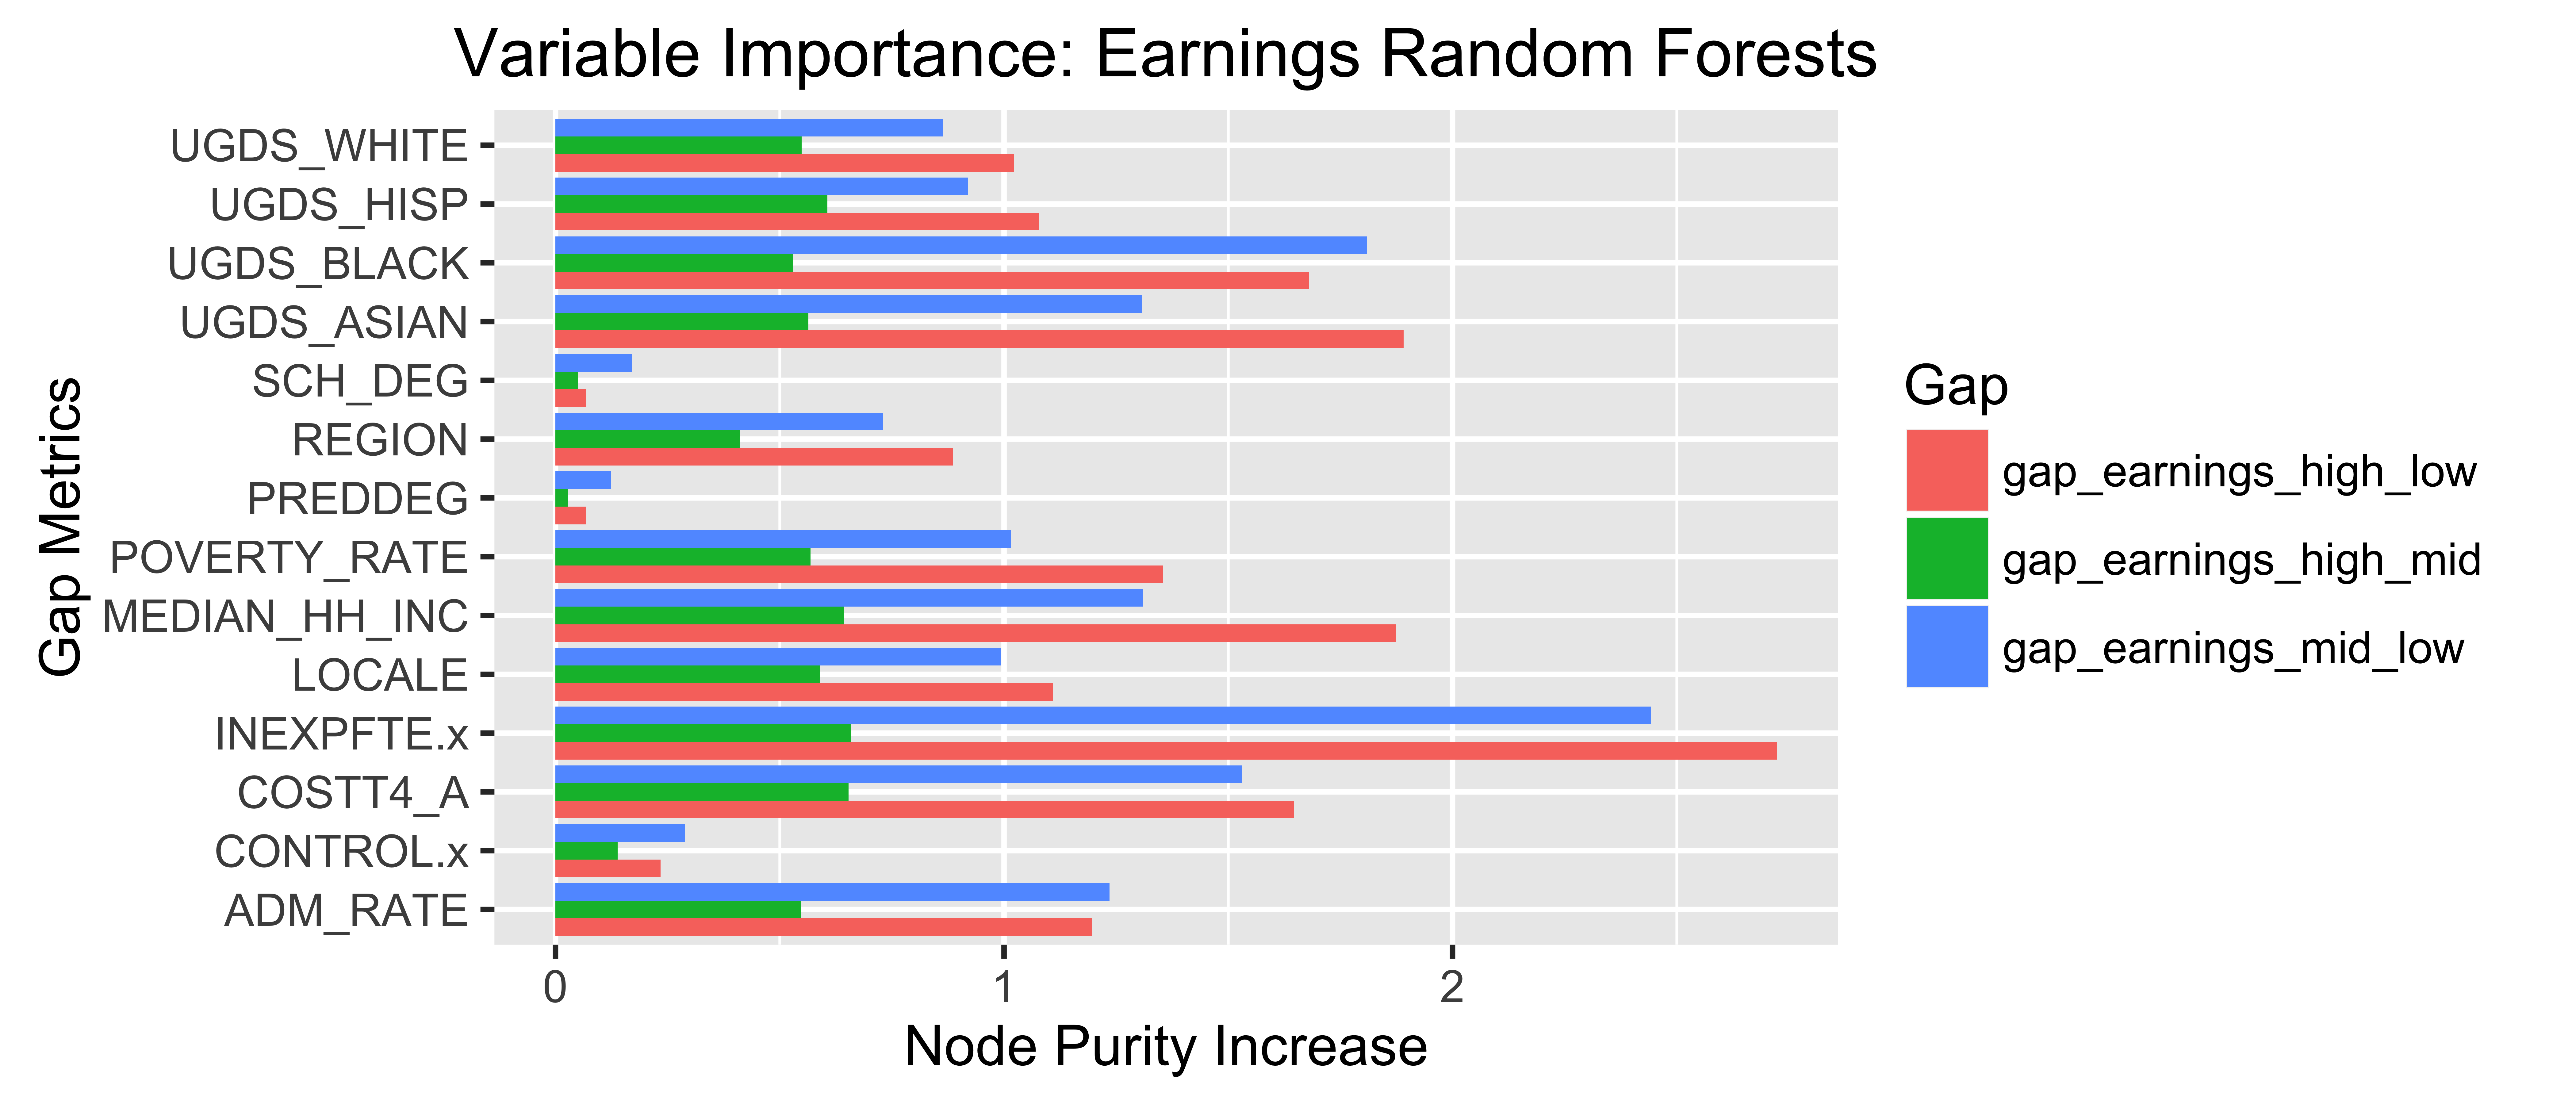
\includegraphics[width=0.5\textwidth]{../images/rf_importance_earnings.png}
\caption{\label{fig: EarningsRFImportance} Here again, we see that INEXPFTE is the strongest variable for the best performing model, high low. We also notice that Median Household Income and Cost to Attend are stronger in these models, which intutitively makes sense given that we are comparing groups according to parent income. Interestingly, UGDSBLACK and UGDSASIAN are fairly important as well.}
\end{figure}

Relating these results to our previous analysis, we find that overall, Expenditures per Student seems to have a stronger relationship with outcome gaps than most other variables, while CONTROL is actually consistently one of the weakest variables. 


\end{document}
